\section{Introduction}

% CUE 3 | 0:50 | 산술평균의 착시와 변동성 항력
\begin{frame}{다기간 투자의 현실: 산술평균의 착시와 변동성 항력}
\begin{columns}[T]
  \begin{column}{0.48\textwidth}
    \textbf{전통 포트폴리오 이론의 구조적 맹점}
    \begin{itemize}
      \setlength{\itemsep}{5pt}
      \item \textbf{단일기간 정적 가정 (Markowitz, 1952)}:
      기대수익률을 단순 \textbf{산술평균($\mu$)}으로 취급.
      \item \textbf{다기간 연속 복리 투자의 실상}:
      장기 부($W_T$)의 축적은 \textbf{기하평균($g$)}이 지배.
      \item \textbf{자본 잠식 예시 (+50\%와 -50\%의 반복)}:
      \begin{align*}
        \mu &= \frac{+50\% - 50\%}{2} = \mathbf{0.0\%} \quad \text{(산술평균)} \\
        g &= \sqrt{1.5 \times 0.5} - 1 = \mathbf{-13.4\%} \quad \text{(기하평균)}
      \end{align*}
      \item 매 사이클마다 \textbf{$-13.4\%p$}의 자본이 허공으로 증발 $\rightarrow$ \textbf{변동성 항력(Volatility Drag)}
    \end{itemize}
  \end{column}
  
  \begin{column}{0.50\textwidth}
    \centering
    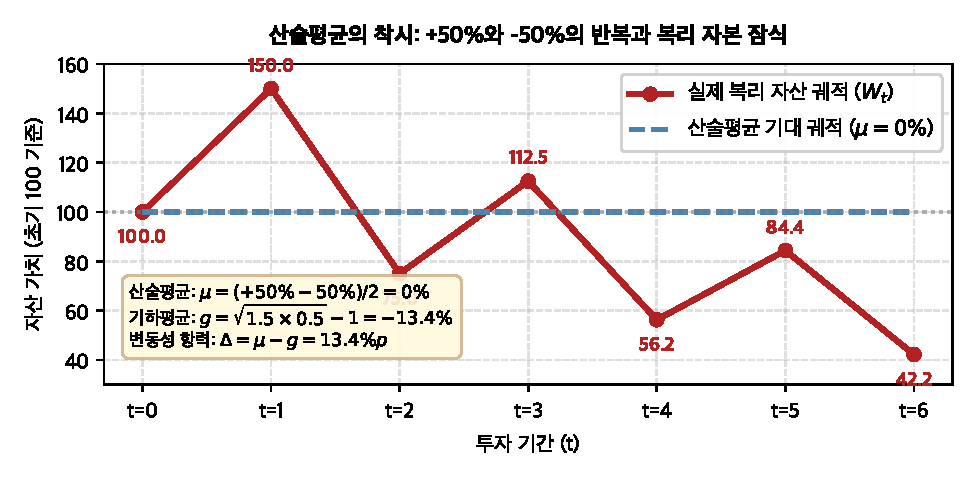
\includegraphics[width=\linewidth]{MyFigure/arith_vs_geom.pdf}
    \vspace{-2mm}
    \begin{block}{핵심 문제의식}
      \small 분산($\sigma^2$)은 단순한 리스크 측정치가 아니라, 시간 축 위에서 기하급수적으로 자본을 갉아먹는 \textbf{실재하는 마찰 비용}이다.
    \end{block}
  \end{column}
\end{columns}
\end{frame}

% CUE 4 | 0:45 | 연구 질문과 3대 기여도
\begin{frame}{연구 질문 및 본 연구의 3대 핵심 기여도}
\begin{block}{핵심 연구 질문 (Core Research Question)}
  \centering
  \large \textit{"자산의 변동성 항력($\frac{1}{2}\sigma^2$)을 사전적으로 통제하고, 극단적 꼬리위험을 차단하여 장기 실질 복리 자본 축적을 극대화할 수 있는가?"}
\end{block}

\vspace{3mm}

\begin{columns}[T]
  \begin{column}{0.32\textwidth}
    \textbf{1. 이론적 기여 (Theoretical)}
    \begin{itemize}
      \setlength{\itemsep}{3pt}
      \small
      \item 이토 보조정리를 코어로 배치
      \item 켈리 기준($\lambda=1$) 하에서 다변량 복리 성장률 직접 목적함수화
      \item 에르고딕성 붕괴 규명
    \end{itemize}
  \end{column}
  
  \begin{column}{0.32\textwidth}
    \textbf{2. 방법론적 기여 (Methodological)}
    \begin{itemize}
      \setlength{\itemsep}{3pt}
      \small
      \item TSFM(Chronos/PatchTST) 제로샷 확률 모멘트 추정
      \item 르두아-울프 + 하이엄 PSD 복원
      \item 산업 비파괴검사(NDE) 기반 비지도 오토인코더 세이프가드
    \end{itemize}
  \end{column}
  
  \begin{column}{0.32\textwidth}
    \textbf{3. 정책적 기여 (Practical)}
    \begin{itemize}
      \setlength{\itemsep}{3pt}
      \small
      \item 국민연금(NPS) 산술평균 착시 극복 및 수지적자 자산 매각 방어
      \item ALM `동적 변동성 예산제' 제안
      \item 퇴직연금 디폴트옵션 TDF 알고리즘 혁신
    \end{itemize}
  \end{column}
\end{columns}
\end{frame}
